% ===================================================================
% Arquivo: capitulos/parte-III-pilares/cap-07-sigmoidais.tex
% ===================================================================

\chapter{Funções de Ativação Sigmoidais}
\label{cap:ativacao-sigmoidais}

% ===================================================================
% Resumo do capítulo
% ===================================================================

% ===================================================================
% Teoremas da Aproximação Universal
% ===================================================================

\section{Teoremas da Aproximação Universal}

Pense que você tem uma função matemática, como $f(t) = 40t + 12$, a qual representa o deslocamento em quilˆmetros de um carro em uma cidade, onde $t$ é o tempo em horas. Caso você queira encontrar o valor de deslocamento quando o carro tiver andando por 3 horas, basta substituir a variável $t$ por 3 e resolver a expressão. Assim temos:

\[\begin{WithArrows}
    f(t) & = 40t + 12 \Arrow{Quando t = 3} \\
    f(3) & = 40\cdot 3 + 12 = 132 km
\end{WithArrows}\]

Esse cenário é o mais comum quando estamos estudando, contudo existe um segundo cenário que também é possível de acontecer. Isso ocorre quando temos um conjunto de pontos e, com base neles, queremos encontrar uma função que descreva o comportamento desses pontos.

Pense que temos os pontos dispostos no gráfico da figura \ref{fig: pontos_addplot} e queremos encontrar uma reta que tente passar o mais próximo de cada um deles.

\begin{figure}[h!]
    \centering
    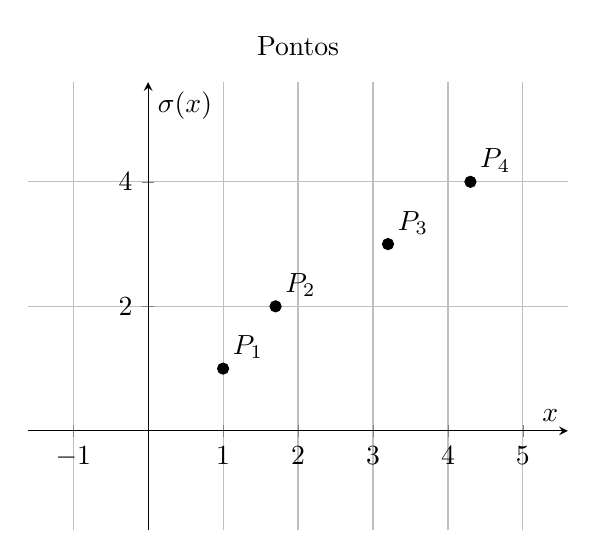
\begin{tikzpicture}
        \begin{axis}[
            title={Pontos},
            xlabel={$x$},
            ylabel={$\sigma(x)$},
            xmin=-1, xmax=5,
            ymin=-1, ymax=5,
            axis lines=middle,
            grid=major,
            enlarge x limits=0.1, 
            enlarge y limits=0.1,
        ]
        \addplot[
            only marks,                     
            mark=*,                       
            mark size=2pt,              
            nodes near coords,             
            point meta=explicit symbolic,   
            nodes near coords align={above right}, 
        ] table [meta=label] { 
            x y label
            1 1 $P_1$
            1.7 2 $P_2$
            3.2 3 $P_3$
            4.3 4 $P_4$ 
        };
        \end{axis}
    \end{tikzpicture}
    \caption{Conjunto de pontos dispostos no plano cartesiano.}
    \label{fig: pontos_addplot}
\end{figure}

Existe uma técnica que permite que nos façamos isso, ela se chama \textbf{regressão linear} (a qual é um dos tópicos discutidos no capítulo \ref{cap:regressao}), e com base nela, é possível dado um conjunto de pontos em um plano, traçar uma reta que se aproxime igualmente de cada um desses pontos. Existem diferentes técnicas de regressão linear, neste caso aplicaremos a dos mínimos quadrados e encontramos a expressão:

\[ y=0.8623x+0.3011 \]

Com base nessa função que encontramos, podemos desenhá-la junto ao gráfico dos pontos e vermos se ela é realmente uma boa aproximação, assim temos a figura \ref{fig: regressao-linear}

\begin{figure}[h!]
    \centering
    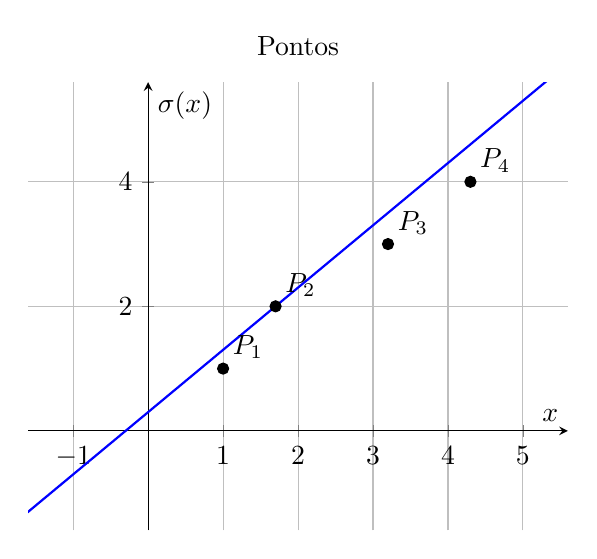
\begin{tikzpicture}
        \begin{axis}[
            title={Pontos},
            xlabel={$x$},
            ylabel={$\sigma(x)$},
            xmin=-1, xmax=5,
            ymin=-1, ymax=5,
            axis lines=middle,
            grid=major,
            enlarge x limits=0.1, 
            enlarge y limits=0.1,
        ]
        \addplot[
            only marks,                     
            mark=*,                       
            mark size=2pt,              
            nodes near coords,             
            point meta=explicit symbolic,   
            nodes near coords align={above right}, 
        ] table [meta=label] { 
            x y label
            1 1 $P_1$
            1.7 2 $P_2$
            3.2 3 $P_3$
            4.3 4 $P_4$ 
        };
        \addplot[blue, thick, domain=-8:8, samples=100] {0.8623(x) + 0.3011};
        \end{axis}
    \end{tikzpicture}
    \caption{Conjunto de pontos dispostos no plano cartesiano.}
    \label{fig: regressao-linear}
\end{figure}

Existem diversas aproximações além da regressão linear, se quisermos, podemos tentar aproximar esses pontos utilizando uma função quadrática, cúbica ou até mesmo exponencial.

Esse tema parece não ter uma conexão com esse capítulo de funções de ativação, mas na realidade, o que muitas das vezes é feito por uma rede neural é justamente esse trabalho de encontrar uma função que aproxima o comportamento de um conjunto de pontos. Só que neste caso, não teremos um conjunto de pontos, vamos ter várias informações em uma base de dados, como imagens de exames médicos ou informações sobre o valor de imóveis e queremos encontrar de alguma forma uma conexão entre esses dados.

Para isso, existe um conjunto de teoremas que servem justamente para provar que uma determinada rede neural criada será capaz de encontrar uma função que descreva o comportamento que você esteja estudando. Eles são os teoremas da aproximação universal.

No livro \textit{Deep Learning}, \textcite{DeepLearningBook} dedicam uma seção explicando esses teoremas. Segundo os autores, o teorema da aproximação universal, introduzido \textcite{Cybenko1989} para a comunidade científica no texto \textit{Approximation by Superpositions of a Sigmoidal Function}, afirma que uma rede feedforward com uma camada de saída linear e no mínimo uma camada oculta com qualquer função que possui a propriedade de "esmagamento", como a sigmoide logística, é capaz de aproximar qualquer função mensurável de Borel de um espaço de dimensão finita para outro com qualquer quantidade de erro diferente de zero desejada desde que essa rede neural possua unidades ocultas suficientes.

Para entendermos esse teorema, devemos primeiro entender o conceito de mensurabilidade de Borel, segundo \textcite{DeepLearningBook} uma função contínua em um subconjunto fechado e limitado de $\mathcal{R}^N$ é mensurável por Borel. Assim esse tipo de função pode ser aproximada por uma rede neural. Além disso, os autores ressaltam que por mais que o teorema original tenha conseguido provar apenas para as funções que saturam tanto para termos muito negativos ou termos muito positivos, diversos outros autores como \textcite{Leshno1993}, no texto \textit{Multilayer feedforward networks with a nonpolynomial activation function can approximate any function}, foram capazes de provar que o teorema da aproximação universal pode funcionar para outras funções, no caso de Leshno, eles provaram para funções não polinomiais, como a Rectified Linear Unit (ReLU), a qual é o tema central do capítulo \ref{cap:ativacao-retificadoras}.

Basicamente os teoremas da aproximação universal reforçam o uso de funções de ativação para permitir que as redes neurais resolvam os problemas propostos por meio da aproximação de uma função. Isso acontece porque essas funções introduzem a não linearidade para a rede, como nos vimos na equação do neurônio de uma rede neural, uma RNA é composta por diferentes camadas de neurônios que são capazes de pegar valores de entrada, multiplicar por um peso dado e somar com um viés, esse resultado passa então por uma função de ativação.

\[ y = x \cdot w + b\]

Se nos tivéssemos uma rede neural em que os neurônios não possuíssem uma função de ativação, ou, fosse uma função linear, mesmo juntando todas essas camadas de neurônios que trazem expressões lineares, a junção disso, ainda seria uma expressão linear. Mas quando introduzimos uma função não linear, como a sigmoide, o teorema da aproximação universal, nos garante que somos capazes de encontrar qualquer função que estivermos procurando, desde que ela seja mensurável de Borel.

\section{Exemplo Ilustrativo: Empurrando para extremos}

Imagine que você está trabalhando para uma empresa na área de marketing e precisa analisar como foi a recepção do público para um novo produto anunciado. Para isso, você ficou responsável por classificar os comentários do público sobre esse produto. Você precisa colocar eles em duas categorias: avaliação positiva ou negativa. Então você precisa ler cada comentário e colocar ele em uma dessas categorias. 

No começo foi fácil, mas depois de um tempo foi ficando repetitivo, então você teve a ideia de automatizar esse processo. Assim, você decide criar um diagrama de uma “caixa-preta” responsável por classificar automaticamente esses comentários da mesma forma que estava fazendo. Essa “caixa” irá receber uma entrada, neste caso, o texto do comentário sobre o produto, e irá retornar uma saída, uma classificação positiva ou negativa sobre o comentário. 

Na matematica, as funções do tipo sigmoide são excelentes para esse tipo de problema, pois possuem uma propriedade muito interessante: dado um valor de entrada, elas são capazes de "empurrar" esse valor para dois diferentes extremos. No caso da sigmoide logísitca, a função que dá nome a essa família, ela é capaz de empurrar essa entrada para valores próximos de zero ou um. Se nós consideramos que zero é uma avaliação negativa e um é uma avaliação positiva, essa função se torna perfeita para resolver o seu problema de classificar comentários.

\section{A Sigmoide Logística}

Por mais que a sigmoide hoje em dia seja bem comum em redes neurais, seu uso não começou nesse cenário. A sigmoide tem suas origens a analise de crescimento populacional e demografia, ela nao surgiu em um artigo em especifico, sendo mais uma evolução presente em vários artigos do matemático belga Pierre François Verhulst dentre os anos de 1838 e 1847. Contudo, existe um artigo desse matemático, intitulado \textbf{"Recherches mathématiques sur la loi d'accroissement de la population"} (Pesquisas matemáticas sobre a lei de crescimento da população), em que Verhulst propõem a função logística como um modelo para descrever o crescimento populacional, levando em consideração a capacidade de suporte de um ambiente, isso gerou a curva em "S" característica da sigmoide. Contudo, foi somente no próximo século, que sigmoide passou a ser utilizada na area da ciência da computação.

\section{Contexto Histórico: Popularização da Sigmoide em Redes Neurais}

A primeira familia de funções que iremos conhecer são as sigmodais, sendo a principal delas, e que da nome a essa família a sigmoide logística. Para isso, vamos entender o contexto em que elas se popularizaram.

Nos anos 1980, estavam ocorrendo mudanças com as funções que eram utilizadas para construir uma rede neural, um desses motivos foi a introdução da retropropagação pelos pesquisadores Daviel Rumelhart, Geoffrey Hinton e Ronald Williams. A retropropagação era uma técnica que permitia que um modelo aprendesse com base nos seus erros, ajustando automaticamente os seus parâmetros em busca de conseguir uma melhor acurácia. 

Além disso, na pesquisa que introduz a retropropagação, \textbf{"Learning representations by back-propagating errors"} de 1986, os cientistas propõem o uso da função sigmoide logística como uma das candidatas para ser utilizada junto com a retropropagação como uma função de ativação. Como justificativa, eles citam o fato dela ser uma função que é capaz de introduzir a não-linearidade para o modelo, permitindo que ele aprenda padrões mais complexos, e também por possui uma derivada limitada.

Mas esse não foi o único fator que fez com que a sigmoide e sua familia se tornassem funções populares para a época. Pouco antes da criação da retropropagação, na década passada, haviam cientistas estudando o comportamento dos neurônios humanos como inspiração para a criação de redes neurais artificiais. Um exemplo desse caso foi o dos cientistas Wilson Hugh e Jack Cowan, em 1972 eles publicaram um artigo intitulado \textbf{"excitatory and Inhibitory interactions in localized populations of model neurons"}, em que buscam estudar como os neurônios respondiam a determinados estímulos.

No artigo, Hugh e Cowan buscam analisar o comportamento de populações localizadas de neurônios excitatórios (denotados pela função $E(t)$) e inibitórios (representados por $I(t)$) e como as duas interagem entre si. Para isso, eles utilizam como variável a proporção de células em uma subpopulação que dispara/reage por unidade de tempo. Para modelar essa atividade eles fizeram o uso uma variação da função sigmoide, representada para expressão \ref{eq: EquacaoNeuronio}, que era capaz de descrever o comportamento dos neurônios a certos estímulos.

\begin{equacaodestaque}{Neurônio de Wilson e Cowan}
    \mathcal{S}(x) = \frac{1}{1 + e^{-a(x - \theta)}} - \frac{1}{1 + e^{a\theta}}
    \label{eq:neuronio-de-wilson-cowan}
\end{equacaodestaque}


Nessa equação, o parâmetro $a$ representa a inclinação, a qual foi ajustada para passar pela origem ($\mathcal{S}(0) = 0$) e $\theta$ 
é o limiar. Para o plotar o gráfico da figura \ref{fig: ComportamentoNeuronios}, foi utilizado os mesmos valores escolhidos pelos cientistas na pesquisa, assim $a = 1.2$ e $\theta = 2.8$.

\begin{figure}[h!]

    \pgfmathdeclarefunction{wilson_sigmoid}{3}{% 
        \pgfmathparse{1/(1+exp(-#1*(#3-#2))) - 1/(1+exp(#1*#2))}%
    }

    \centering
    \begin{tikzpicture}
        \begin{axis}[
            title={Função Sigmoide de Wilson-Cowan},
            xlabel={$x$ (Estímulo)},
            ylabel={$s(x)$ (Proporção de Ativação)},
            xmin=-2, xmax=10, % Ajusta o eixo x para centralizar a curva
            ymin=-0.1, ymax=1.1, % Ajusta o eixo y
            axis lines=middle,
            grid=major,
            legend pos=north west,
            % Define os parâmetros para a função
            /pgf/declare function={a=1.2; theta=2.8;}
            ]
            \addplot[blue, thick, domain=-2:10, samples=150] {wilson_sigmoid(a, theta, x)};
        \end{axis}
    \end{tikzpicture}
    \caption{Gráfico da função sigmoide conforme proposta por Wilson e Cowan (1972), com parâmetros de exemplo $a=1.2$ e $\theta=2.8$.}
    \label{fig: ComportamentoNeuronios}
\end{figure}

Os cientistas demonstram que a população de neurônios reage de formas distintas quando sofrem determinados estímulos. Os níveis baixos de excitação não conseguem ativar a população, porém, existe uma região de alta sensibilidade, na qual pequenos aumentos no estímulo geram um grande aumento na atividade. Além disso, existe um terceiro nível, o de saturação, em que níveis muito altos de estímulos são capazes de ativar todas as células e a partir disso, a resposta da população atinge o comportamento de uma função constante, indicando que ela saturou. Ao juntar todos esses três níveis, temos a famosa curva em "S", caraterística da função sigmoide.

\begin{figure}[h!]
    \centering
    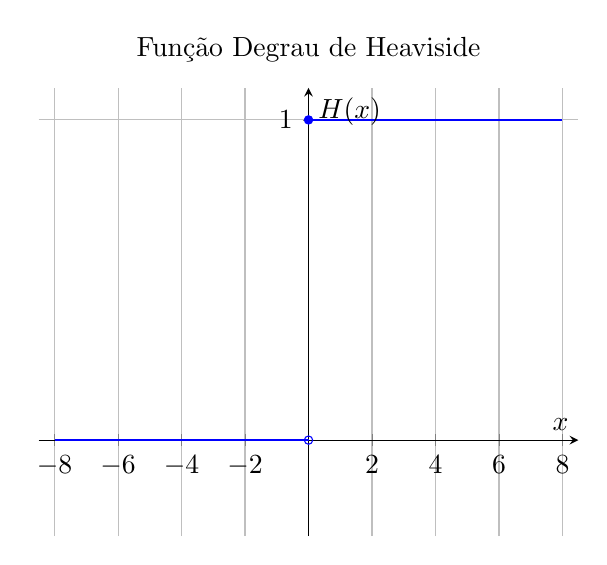
\begin{tikzpicture}
        \begin{axis}[
            title={Função Degrau de Heaviside},
            xlabel={$x$},
            ylabel={$H(x)$},
            xmin=-8.5, xmax=8.5,
            ymin=-0.3, ymax=1.1,
            axis lines=middle,
            grid=major,
            ytick={0,1}, % Define os ticks no eixo y para 0 e 1
        ]
        % Desenha a parte da função para x < 0
        \addplot[blue, thick, domain=-8:0] {0};
        % Desenha a parte da função para x >= 0
        \addplot[blue, thick, domain=0:8] {1};

        % Adiciona os marcadores para a descontinuidade em x=0
        % Círculo aberto em (0,0) para indicar que o ponto não pertence a essa parte
        \addplot[only marks, mark=o, mark size=1.5pt, blue, fill=white] coordinates {(0,0)};
        % Círculo fechado em (0,1) para indicar que o ponto pertence a essa parte
        \addplot[only marks, mark=*, mark size=1.5pt, blue] coordinates {(0,1)};
        \end{axis}
    \end{tikzpicture}
    \caption{Gráfico da função degrau de Heaviside.}
    \label{fig:degrau-unitario}
\end{figure}

Com isso, ao consideramos esses dois cenários: a criação da retropropagação e busca na natureza para inspiração na criação de redes neurais. A sigmoide, junto com a sua família, se tornaram funções muito populares para a época, estando presentes em varias redes neurais criadas. Um desses exemplos é a rede de Elman, um tipo de rede neural recorrente criada para aprender e representar estruturas em dados sequenciais. Elman cita em seu estudo \textbf{"Finding structure in time"} de 1990 que era ideal o uso de uma função de ativação com valores limitados entre zero e um, um cenário ideal para o uso da sigmoide.

Cabe destacar também que, as sigmodais nao foram as primeiras funções de ativação a serem utilizadas na criação de uma rede neural. Nesse cenário de redes neurais, existem sempre funções que são mais populares, e que com o tempo e o surgimento de novas pesquisas, são deixadas de lado para novamos funções mais interessantes.

Uma função que era muito utilizada era a heavside, ou degrau em português. Ela inclusive esteve presente na produção da rede neural Perceptron criada por Frank Rosenblatt e introduzida para a comunidade científica no artigo \textbf{"The Perceptron: A probabilistic model for informations storage and organization in the brain"} em 1958.

Quando a comparamos a degrau unitário com a sigmoide, notamos uma diferença crucial, a sigmoide é uma função contínua em todos os pontos, podemos dizer que para desenhar seu gráfico não precisamos tirar o lápis do papel nenhuma vez, algo que não ocorre com a heavside. Além disso, a derivada da heavside é zero em quase todos os seus pontos, por esse motivo, ela impossibilitava a retropropagação do erro, uma vez que quando fossemos calcular o gradiente para uma parte de um modelo que usasse essa função, ele provavelmente seria zero.

Por mais que a sigmoide hoje em dia seja bem comum em redes neurais, seu uso não começou nesse cenário. A sigmoide tem suas origens a analise de crescimento populacional e demografia, ela nao surgiu em um artigo em especifico, sendo mais uma evolução presente em vários artigos do matemático belga Pierre François Verhulst dentre os anos de 1838 e 1847. Contudo, existe um artigo desse matemático, intitulado \textbf{"Recherches mathématiques sur la loi d'accroissement de la population"} (Pesquisas matemáticas sobre a lei de crescimento da população), em que Verhulst propõem a função logística como um modelo para descrever o crescimento populacional, levando em consideração a capacidade de suporte de um ambiente, isso gerou a curva em "S" característica da sigmoide. Contudo, foi somente no próximo século, que sigmoide passou a ser utilizada na area da ciência da computação.

\begin{equacaodestaque}{Sigmoide Logística}
    \sigma(z_i) = \frac{1}{1 + e^{-z_i}}
    \label{eq:sigmoide}
\end{equacaodestaque}

\begin{figure}[h!]
    \centering
    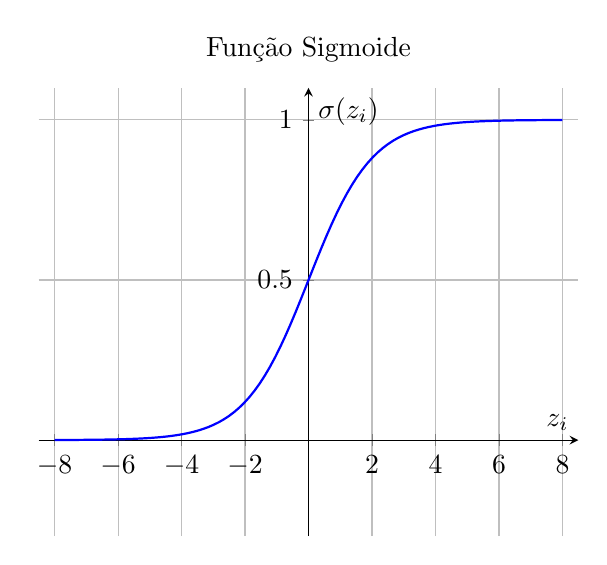
\begin{tikzpicture}
        \begin{axis}[
            title={Função Sigmoide},
            xlabel={$z_i$},
            ylabel={$\sigma(z_i)$},
            xmin=-8.5, xmax=8.5,
            ymin=-0.3, ymax=1.1,
            axis lines=middle,
            grid=major,
        ]
        \addplot[blue, thick, domain=-8:8, samples=100] {1/(1+exp(-x))};
    \end{axis}
    \end{tikzpicture}
    \caption{Gráfico da função sigmoide logística.}
    \label{fig: GraphSigmoid}
\end{figure}

A função sigmoide é escrita com uma exponencial, como na fórmula \ref{eq: FormulaSigmoide}. Johannes Lederer, no texto \textbf{"Activations Functions in Artificial Neural Networks: A Systematic Overview"}, explica sobre a sigmoide, segundo o autor, ela é uma função limitada, diferenciável e monotônica, o que significa que conforme os valores de $x$ aumentam os valores de $f(x)$ também aumentam.

Como vemos na figura \ref{fig: GraphSigmoid}, o gráfico da sigmoide possui o formato de um "S" deitado. Assim, também podemos dizer que a função sigmoide é uma função suave, contínua (o que a possibilita de ser derivável em todos os pontos) e também é não linear. Lederer explica que uma das propriedades interessantes da sigmoide está no fato dela empurrar os valores de entrada para dois extremos, neste caso, 0 e 1.

Note que, conforme os valores crescem/decrescem muito, essa curva passa a assumir o comportamento de quase uma reta, tendo pouca variação entre esses valores, esse ponto será discutido mais em seguida.

Agora podemos discutir a sua derivada, para resolvê-la, podemos aplicar uma regra do quociente obtendo a expressão \ref{eq: DerivadaSigmoide} e o gráfico \ref{fig: GraphSigmoidDerivada}

\begin{equacaodestaque}{Derivada da sigmoide logística}
    \frac{d}{dz_i}\sigma(z_i) = \frac{e^{-z_i}}{(1 + e^{-z_i})^2}
    \label{eq:sigmoide-derivada}
\end{equacaodestaque}

\begin{figure}[h!]
    \centering
    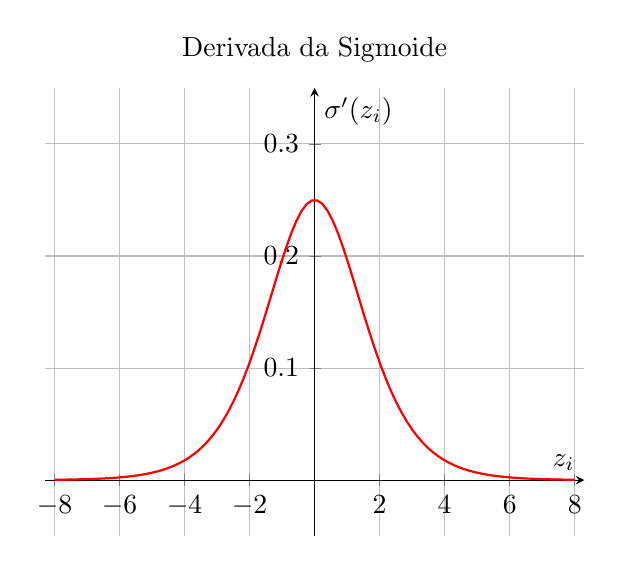
\begin{tikzpicture}
        \begin{axis}[
            title={Derivada da Sigmoide},
            xlabel={$z_i$},
            ylabel={$\sigma'(z_i)$},
            xmin=-8.3, xmax=8.3,
            ymin=-0.05, ymax=0.35,
            axis lines=middle,
            grid=major,
        ]
        \addplot[red, thick, domain=-8:8, samples=100] {exp(-x)/((1+exp(-x))^2)};
        \end{axis}
    \end{tikzpicture}
    \caption{Gráfico da derivada da sigmoide.}
    \label{fig: GraphSigmoidDerivada}
\end{figure}

Notamos que sua derivada é contínua em todos os pontos e que ela atinge um ponto máximo entre 0.2 e 0.3 e que para valores que passam de $\pm 8$ os resultados serão muito próximos de zero, isso acontece pois, como vemos no gráfico \ref{fig: GraphSigmoid}, a própria função sigmoide, não apresenta muita variação de valores conforme eles ultrapassam $\pm 8$. Guarde essa informação, pois ela sera necessária para entender o conceito de gradiente evanescente, que será explicado no fim do capitulo. Contudo, a derivada da sigmoide também pode ser expressa em termos da própria sigmoide como a equação \ref{eq: DerivadaSigmoideVariacao} nos mostra.

Ao analisarmos a derivada da sigmoide na expressão \ref{eq: DerivadaSigmoideVariacao} vemos que ela possui uma derivada bem elegante e atrativa para as os cientistas da computação da época, pois pelo fato dela poder ser escrita em termos de sua própria função, isso permite que vários cálculos possam ser reaproveitados. Isso é algo interessante para a criação de uma rede neural no milênio passado pois, devemos lembrar que os computadores da época não possuíam uma poder computacional tão alto como os da atualidade. Assim, qualquer calculo que pudesse ser reaproveitado e até mesmo simplificado, já era de muita ajuda para os cientistas além de poupar grande tempo de processamento.

\textbf{Implementação em Python}

Com base nesses dados, podemos escrever a sua implementação em código. Para isso, devemos apenas seguir a fórmula da sigmoide logística e sua derivada. Temos então o bloco de código \ref{lst:codigo-sigmoide}.

\begin{codelisting}{Classe completa do função de ativação Sigmoid}{gd_class}
import numpy as np

class Sigmoid(Layer):
    def __init__(self):
        super().__init__()
        self.input = None
        self.sigmoid = None

    def forward(self, input_data):
        self.input = input_data
        self.sigmoid_output = 1/ (1 + np.exp(-input_data))
        return self.sigmoid_output

    def backward(self, grad_output):
        sigmoid_grad = self.sigmoid_output * (1 - self.sigmoid_output)
        return grad_output * sigmoid_grad, None
\end{codelisting}

\section{Tangente Hiperbólica}

Assim como a função sigmoide, a tangente hiperbólica não possui suas origens voltadas para o uso em redes neurais. Neste caso, um dos matemáticos que ficou reconhecido por criar a notação das funções hiperbólicas, seno, cosseno e tangente, foi o suíço Johann Heinrich Lambert no trabalho de 1769 \textbf{"Mémoire sur quelques propriétés remarquables des quantités transcendantes circulaires et logarithmiques"} (Memória sobre algumas propriedades notáveis de grandezas transcendentais circulares e logarítmicas), em que provou que muitas das identidades trigonométricas possuíam suas equivalentes hiperbólicas.

Passando mais de dois séculos, a tangente hiperbólica já estava sendo utilizada em diversas redes neurais, ela inclusive fez parte da primeira rede neural convolucional criada, estando presente na Le-Net-5, uma rede neural criada para identificar e classificar imagens de cheques em caixas eletrônicos. No artigo acadêmico \textbf{"Gradient-based learning applied to document recognition"} de 1998, os cientistas Yann LeCun, Léon Bottou, Yousha Bengio e Patrick Haffner explicam a criação dessa rede além de destacar suas métricas alcançadas.

Semelhante a sigmoide, a tangente hiperbólica possui várias propriedades parecidas. Como afirma Lederer em \textbf{"Activation Functions in Artificial Neural Networks: A Systematic Overview"} a tangente hiperbólica é infinitamente diferenciável, sendo uma versão escalada e rotacionada da sigmoide logística. Assim, como podemos ver no gráfico da figura \ref{fig: GraphTanh}, ela é uma função que está centrada em zero, e seus valores variam agora em um intervalo de -1 a 1, diferente da sigmoide, que varia somente de 0 a 1.

Podemos escrever a tangente hiperbólica utilizando a definição de tangente, que é o quociente a função seno com a função cosseno, só que neste caso usaremos as funções hiperbólicas. Assim temos a expressão \ref{eq: EquacaoTanh} e seu gráfico \ref{fig: GraphTanh}.

\begin{equacaodestaque}{Tangente Hiperbólica}
    \tanh(z_i) = \frac{\sinh(z_i)}{\cosh(z_i)} = \frac{e^z_i - e^{-z_i}}{e^z_i + e^{-z_i}}
    \label{eq:tangente-hiperbolica}
\end{equacaodestaque}

\begin{figure}[h!]
    \centering
    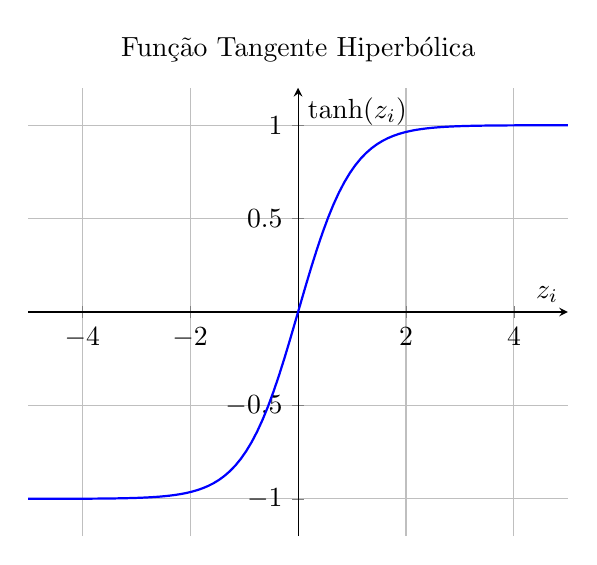
\begin{tikzpicture}
        \begin{axis}[
            title={Função Tangente Hiperbólica},
            xlabel={$z_i$},
            ylabel={$\tanh(z_i)$},
            xmin=-5, xmax=5,
            ymin=-1.2, ymax=1.2,
            axis lines=middle,
            grid=major,
        ]
        \addplot[blue, thick, domain=-5:5, samples=100] {tanh(x)};
        \end{axis}
    \end{tikzpicture}
    \caption{Gráfico da tangente hiperbólica.}
    \label{fig: GraphTanh}
\end{figure}

Agora que temos a expressão da tangente hiperbólica e seu gráfico podemos também calcular sua derivada. Note na expressão \ref{eq: DerivadaTanh}, que podemos escrever a derivada da tangente utilizando a expressão da secante hiperbólica, mas também podemos utilizar a própria tangente hiperbólica se quisermos, assim ela também passa a ser bastante util para reaproveitar códigos e cálculos.

\begin{figure}[h!]
    \centering
    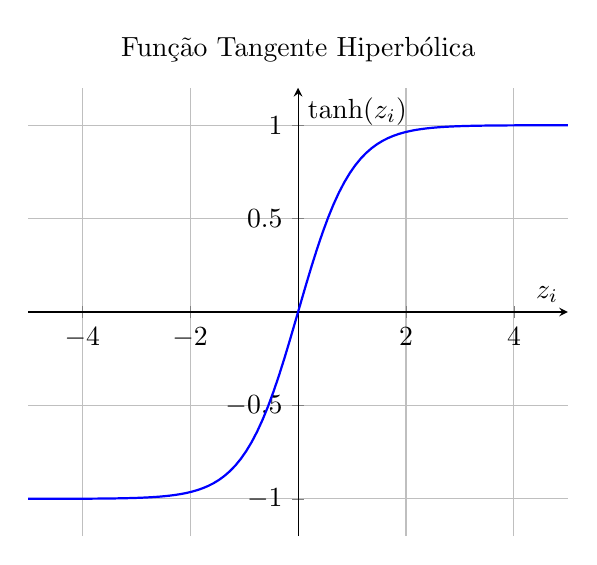
\begin{tikzpicture}
        \begin{axis}[
            title={Função Tangente Hiperbólica},
            xlabel={$z_i$},
            ylabel={$\tanh(z_i)$},
            xmin=-5, xmax=5,
            ymin=-1.2, ymax=1.2,
            axis lines=middle,
            grid=major,
        ]
        \addplot[blue, thick, domain=-5:5, samples=100] {tanh(x)};
        \end{axis}
    \end{tikzpicture}
    \caption{Gráfico da tangente hiperbólica.}
    \label{fig: GraphTanh}
\end{figure}

Semelhante a sigmoide, os valores da tangente hiperbólica também se aproximam de zero conforme aumentam ou diminuem na sua derivada. Eles atingem um pico de 1, e conforme as entradas se aproximam de $\pm 4$ a saída da derivada da tangente hiperbólica também fica próxima de zero. Além disso, como podemos ver na expressão \ref{eq: DerivadaTanhVariacao}, a derivada da tangente hiperbólica também pode ser expressas em termos da sua própria função, permitindo que cálculos possam ser reaproveitados.

\begin{equacaodestaque}{Derivada da tangente hiperbólica}
    \frac{d}{dz_i}\tanh(z_i) = \text{sech}^2(z_i)
    \label{eq:tangente-hiperbolica-derivada}
\end{equacaodestaque}

\begin{figure}[h!]
    \centering
    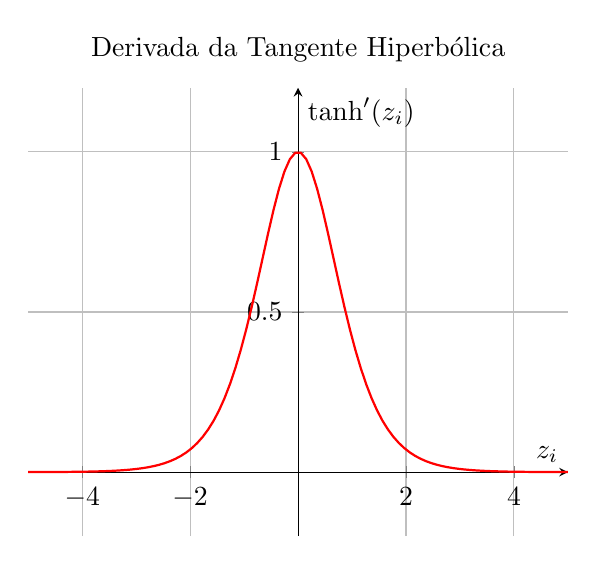
\begin{tikzpicture}
        \begin{axis}[
            title={Derivada da Tangente Hiperbólica},
            xlabel={$z_i$},
            ylabel={$\tanh'(z_i)$},
            xmin=-5, xmax=5,
            ymin=-0.2, ymax=1.2,
            axis lines=middle,
            grid=major,
        ]
        \addplot[red, thick, domain=-5:5, samples=100] {1-(tanh(x))^2};
        \end{axis}
    \end{tikzpicture}
    \caption{Gráfico da derivada da tangente hiperbólica.}
    \label{fig: GraphTanh}
\end{figure}

\textbf{Implementação em Python}

Agora que sabemos como a tangente hiperbólica se comporta, além de conhecermos as suas fórmulas, podemos implementar a sua função em Python, utilizando o numpy para auxiliar nos cálculos.

Para isso, devemos implementar as expressões \ref{eq: EquacaoTanh} e \ref{eq: DerivadaTanh}, obtendo o bloco de código \ref{lst:codigo-tanh}.

\begin{codelisting}{Classe completa do função de ativação Tangente Hiperbólica}{gd_class}
import numpy as np
from layers.base import Layer  # Assuming your base class is here

class Tanh(Layer):
    def __init__(self):
        super().__init__()
        self.input = None
        self.tanh_output = None

    def forward(self, input_data):
        self.input = input_data
        self.tanh_output = np.tanh(self.input)
        return self.tanh_output

    def backward(self, grad_output):
        tanh_grad = 1 - self.tanh_output**2
        return grad_output * tanh_grad, None
\end{codelisting}

\section{Softsign: Uma Sigmoidal Mais Barata}

A próxima função que vamos conhecer é a softsign, diferente da tangente hiperbólica e da sigmoide que tiveram suas origens em outros campos diferentes da ciência da computação, a softsign foi criada com o intuito de ser trabalhada em uma rede neural. Ela foi introduzida no artigo \textbf{"A Better Activation Function for Artificial Neural Networks"} de 1993, do cientista D.L. Elliott. No texto ele propõem a softsign como uma alternativa para as funções sigmodais tradicionais.

Como podemos ver no seu gráfico \ref{fig:GraphSoftsign}, ela possui o formato em "S" característico das sigmodais além de ser centrada em zero como a tangente hiperbólica. Além disso, como Elliot destaca em seu texto, ela é uma função que é diferenciável em toda a reta possuindo também a mesma propriedade das outras sigmodais de empurrar os valores de entrada para os seus extremos. Podemos notar também pelo seu gráfico que ela também uma função contínua, suave e não linear

Contudo, a principal diferença dela com as outras sigmodais está na sua fórmula, como podemos ver na equação \ref{eq:EquacaoSoftsign} ela não utiliza nenhum exponencial para compor sua função. Isso faz com que ela seja uma função mais "barata" em termos de poder computacional para ser implementada em redes neurais. Assim, podemos obter resultados parecidos porem utilizando cálculos menos complexos e com isso teremos redes mais rápidas de serem treinadas. Um comparativo com as funções sigmodais desse texto e como elas reagem poderá ser visto em uma seção futura.

Com base em sua expressão, também podemos plotar o seu gráfico na figura \ref{fig:GraphSoftsign}.

\begin{equacaodestaque}{Softsign}
    \text{softsign}(z_i) = \frac{z_i}{1 + |z_i|}
    \label{eq:softsign}
\end{equacaodestaque}

\begin{figure}[h!]
    \centering
    % Gráfico da função Softsign usando PGFPlots
    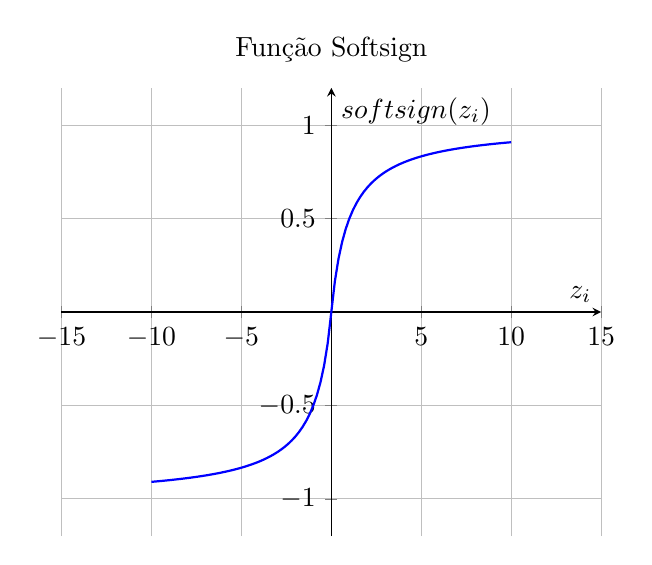
\begin{tikzpicture}
        \begin{axis}[
            title={Função Softsign},
            xlabel={$z_i$},
            ylabel={$\text{softsign}(z_i)$},
            xmin=-15, xmax=15,
            ymin=-1.2, ymax=1.2,
            axis lines=middle,
            grid=major,
        ]
        % A função softsign(x) = x / (1 + abs(x))
        \addplot[blue, thick, domain=-10:10, samples=101] {x / (1 + abs(x))};
        \end{axis}
    \end{tikzpicture}
    \caption{Gráfico da função Softsign.}
\end{figure}

Com relação a sua diferenciabilidade, a softsign pode ser derivada em todos os seus pontos, e sua derivada pode ser vista na expressão \ref{eq:DerivadaSoftsign}. Com base nela, notamos uma outra diferença da softsign com a tangente hiperbólica e a sigmoide. Diferente das outras duas, a derivada da softsign não pode ser expressa em termos da sua própria função. Assim, enquanto nas outras funções é feito um cálculo complexo na função e um simples na derivada, pois aproveitamos o resultado, na softsign isso não ocorre. Podemos pensar que talvez essa função seja mais rápida que as outras duas no Forward, mas não podemos garantir a mesma coisa com relação ao Backward, para isso devemos fazer alguns testes antes.

Podemos ver também no gráfico da derivada da softsign que o valor de sua derivada começa a ficar proximo de zero quando $x$ se aproxima de $\pm 10$, indicando que ela começa a saturar nesse ponto.

\begin{equacaodestaque}{Derivada da softsign}
    \frac{d}{dz_i}\text{softsign}(z_i) = \frac{1}{(1 + |z_i|)^2}
    \label{eq:softsgin-derivada}
\end{equacaodestaque}

\begin{figure}[h!]
    \centering
    % Gráfico da derivada da função Softsign
    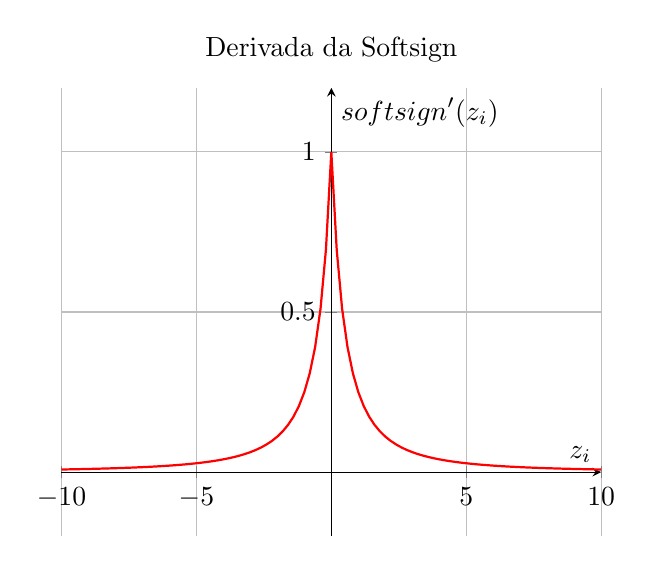
\begin{tikzpicture}
        \begin{axis}[
            title={Derivada da Softsign},
            xlabel={$z_i$},
            ylabel={$\text{softsign}'(z_i)$},
            xmin=-10, xmax=10,
            ymin=-0.2, ymax=1.2,
            axis lines=middle,
            grid=major,
        ]
        % A derivada da softsign é 1 / (1 + |x|)^2
        \addplot[red, thick, domain=-10:10, samples=101] {1/((1+abs(x))^2)};
        \end{axis}
    \end{tikzpicture}
    \caption{Gráfico da derivada da função Softsign.}
    \label{fig:GraphSoftsignDerivative}
\end{figure}

\textbf{Implementação em Python}

Assim, podemos implementar o bloco de código \ref{lst:codigo-softsign} representa a função softsign para ser utilizada uma rede neural.

\begin{codelisting}{Classe completa do função de ativação Softsign}{gd_class}
from layers.base import Layer
import numpy as np

class Softsign(Layer):
    def __init__(self):
        super().__init__()
        self.input = None

    def forward(self, input_data):
        self.input = input_data
        return self.input / (1 + np.abs(self.input))

    def backward(self, grad_output):
        grad =  (1 / (1 + np.abs(self.input))**2)
        return grad_output * softsign_grad, None
\end{codelisting}

\section{Hard Sigmoid e Hard Tanh: O Sacrifício da Suavidade em Prol do Desempenho}

Agora veremos duas funções sigmodais, criadas no contexto de redes neurais, cujo o seu intuito é ser trazer velocidade para o modelo que está sendo criado, elas são a hard sigmoid e hard tanh. Elas são inspiradas nas suas versões originais ou soft, com o mesmo intuito de variar até um certo ponto e depois saturar. Contudo, não garantem a mesma suavidade que as outras funções.

A primeira que vamos ver é a hard sigmoid. Como podemos ver na equação \ref{eq: EquacaoHardSigmoid}, ela pode ser escrita juntando 3 diferentes funções, duas delas sendo funções constantes e uma terceira sendo a função identidade. Note que ela perde a suavidade da função seno, possuindo bicos que a impedem de ser derivada em todos os seus pontos, contudo, seus cálculos são bem mais simples os cálculos quando comparamos com a sigmoide tradicional, não tem nenhuma exponencial para atrasar as respostas da função. Mas note que temos um crescimento linear quando os valores estão entre -3 e 3.

\begin{equacaodestaque}{Hard Sigmoid}
        \text{hard sigmoid}(z_i) = \begin{cases} 0 & \text{se } z_i < -3 \\ z_i/6 + 0.5 & \text{se } -3 \le z_i \le 3 \\ 1 & \text{se } z_i > 3 \end{cases}
    \label{eq:hard-sigmoid}
\end{equacaodestaque}

\begin{figure}[h!]
    \centering
    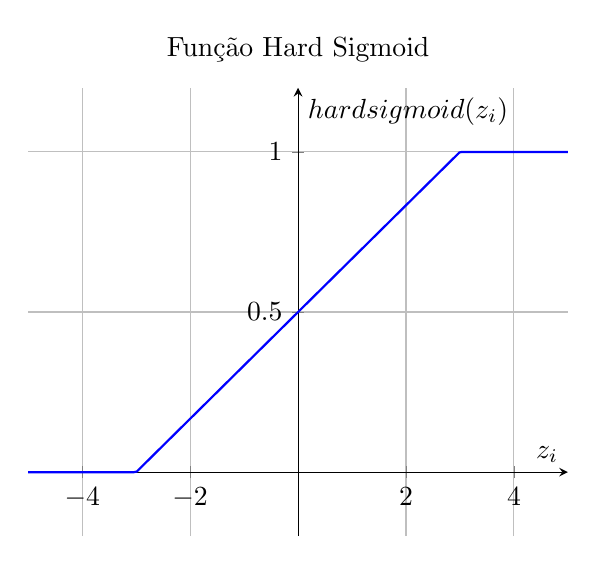
\begin{tikzpicture}
        \begin{axis}[
            title={Função Hard Sigmoid},
            xlabel={$z_i$},
            ylabel={$\text{hard sigmoid}(z_i)$},
            xmin=-5, xmax=5,
            ymin=-0.2, ymax=1.2,
            axis lines=middle,
            grid=major,
            domain=-5:5,
            samples=200, % More samples for a smoother piecewise look
            restrict y to domain*=-0.2:1.2 % Keep plot within y limits
        ]
        % Define the piecewise function using if-else logic for plotting
        \addplot[blue, thick] {
            (x < -3) * 0 +
            (x >= -3 && x <= 3) * (x/6 + 0.5) +
            (x > 3) * 1
        };
        \end{axis}
    \end{tikzpicture}
    \caption{Gráfico da função hard sigmoid.}
    \label{fig: GraphHardSigmoid}
\end{figure}

Com relação a sua derivada, para obtê-lá, apenas derivamos todas as três expressões construindo a expressão da sua derivada. Note que ela também não é suave quando comparamos com a derivada da sigmoide tradicional.

\begin{equacaodestaque}{Derivada da Hard Sigmoid}
        \frac{d}{dz_i}\text{hard sigmoid}(z_i) = \begin{cases} 0 & \text{se } z_i < -3 \\ 1/6 & \text{se } -3 < z_i < 3 \\ 0 & \text{se } z_i > 3 \end{cases}
    \label{eq:hard-sigmoid-derivada}
\end{equacaodestaque}

\begin{figure}[h!]
    \centering
    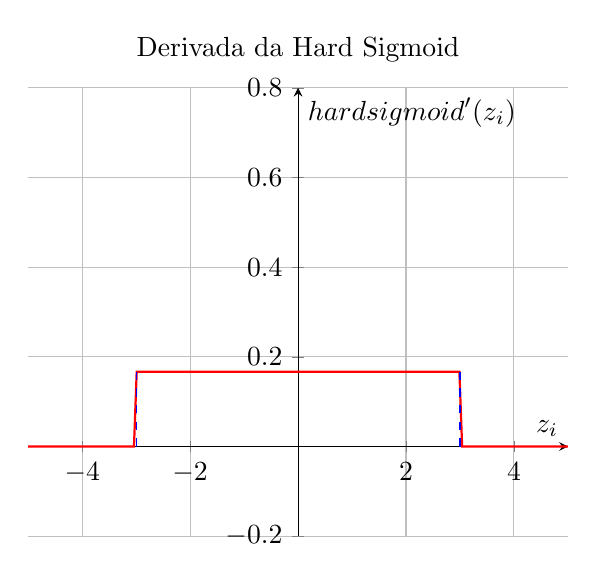
\begin{tikzpicture}
        \begin{axis}[
            title={Derivada da Hard Sigmoid},
            xlabel={$z_i$},
            ylabel={$\text{hard sigmoid}'(z_i)$},
            xmin=-5, xmax=5,
            ymin=-0.2, ymax=0.8,
            axis lines=middle,
            grid=major,
            domain=-5:5,
            samples=200, % More samples to show step clearly
            restrict y to domain*=-0.2:0.8
        ]
        % Plot the derivative: 1/6 between -3 and 3, 0 otherwise
        \addplot[red, thick] {
            (x > -3 && x < 3) * (1/6)
        };
        % Add lines for the jumps (optional, but makes it clearer)
        \draw[dashed, blue] (axis cs:-3, 0) -- (axis cs:-3, 1/6);
        \draw[dashed, blue] (axis cs:3, 0) -- (axis cs:3, 1/6);
        \end{axis}
    \end{tikzpicture}
    \caption{Gráfico da derivada da Hard Sigmoid.}
    \label{fig: GraphDerivadaHardSigmoid}
\end{figure}

Note que o código dessa função é um pouco diferente das outras três que já vimos, ele não faz o uso de IFs, e sim opta por fazer essas operações de forma vetorizada, para garantir que os resultados sejam mais rápidos e otimizados para uma rede neural.

Também temos a função hard tanh, que tem a mesma proposta da hard sigmoid, porém busca imitar a tangente hiperbólica. Ela também é composta de uma condicional com três funções, duas constantes e a função identidade, como podemos ver na equação \ref{eq: EquacaoHardTanh}.

\begin{equacaodestaque}{Hard Tanh}
        \text{hard tanh}(z_i) = \begin{cases} -1 & \text{se } z_i < -1 \\ z_i & \text{se } -1 \le z_i \le 1 \\ 1 & \text{se } z_i > 1 \end{cases}
    \label{eq:hard-tanh}
\end{equacaodestaque}

\begin{figure}[h!]
    \centering
    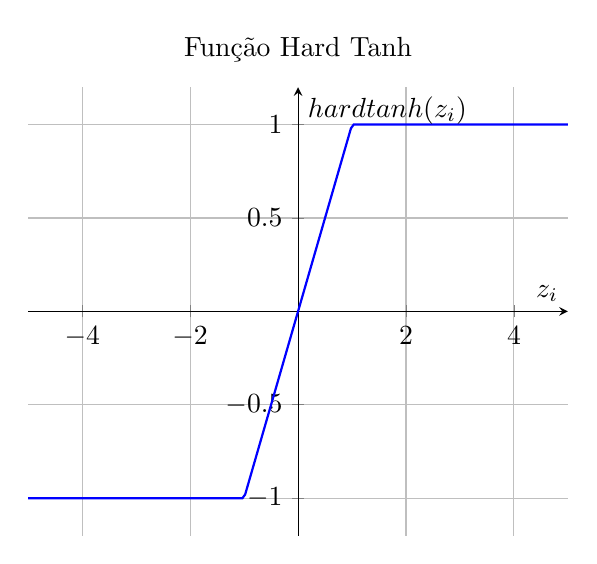
\begin{tikzpicture}
        \begin{axis}[
            title={Função Hard Tanh},
            xlabel={$z_i$},
            ylabel={$\text{hard tanh}(z_i)$},
            xmin=-5, xmax=5,
            ymin=-1.2, ymax=1.2,
            axis lines=middle,
            grid=major,
            domain=-5:5,
            samples=200, % More samples for clarity
            restrict y to domain*=-1.2:1.2 % Keep plot within y limits
        ]
        % Define the piecewise function for plotting
        \addplot[blue, thick] {
            (x < -1) * -1 +
            (x >= -1 && x <= 1) * x +
            (x > 1) * 1
        };
        \end{axis}
    \end{tikzpicture}
    \caption{Gráfico da função Hard Tanh. Fonte: PyTorch.}
    \label{fig: GraphHardTanh}
\end{figure}

Utilizamos o mesmo procedimento da hard sigmoid para obter a derivada da hard tanh, derivamos as três expressões e encontramos então a equação \ref{eq: DerivadaHardTanh}, ao lado, temos a figura \ref{fig: GraphHardTanh}, que representa o gráfico da derivada da hard tanh.

\begin{equacaodestaque}{Derivada da Hard Tanh}
        \frac{d}{dz_i}\text{hard tanh}(z_i) = \begin{cases} 0 & \text{se } z_i < -1 \\ 1 & \text{se } -1 < z_i < 1 \\ 0 & \text{se } z_i > 1 \end{cases}
    \label{eq:hard-tanh-derivada}
\end{equacaodestaque}

\begin{figure}[h!]
    \centering
    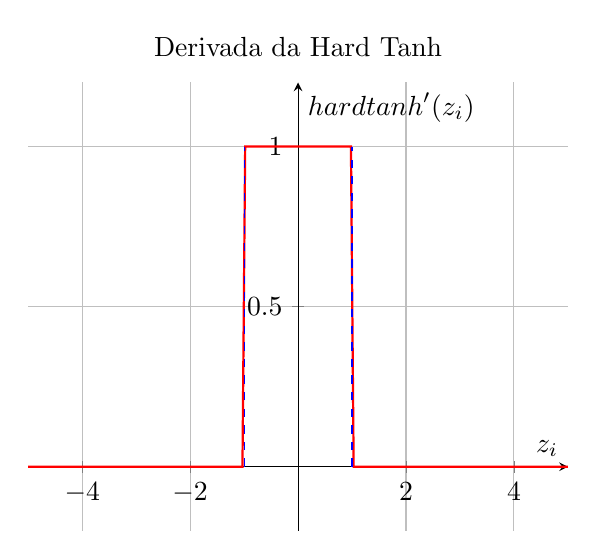
\begin{tikzpicture}
        \begin{axis}[
            title={Derivada da Hard Tanh},
            xlabel={$z_i$},
            ylabel={$\text{hard tanh}'(z_i)$},
            xmin=-5, xmax=5,
            ymin=-0.2, ymax=1.2,
            axis lines=middle,
            grid=major,
            domain=-5:5,
            samples=200, % More samples to show step clearly
            restrict y to domain*=-0.2:1.2
        ]
        % Plot the derivative: 1 between -1 and 1, 0 otherwise
        \addplot[red, thick] {
            (x > -1 && x < 1) * 1
        };
        % Add lines for the jumps (optional, but makes it clearer)
        \draw[dashed, blue] (axis cs:-1, 0) -- (axis cs:-1, 1);
        \draw[dashed, blue] (axis cs:1, 0) -- (axis cs:1, 1);
        \end{axis}
    \end{tikzpicture}
    \caption{Gráfico da derivada da Hard Tanh.}
    \label{fig: GraphDerivadaHardTanh}
\end{figure}

\textbf{Implementação em Python}

Para implementar a hard sigmoid em python, apenas devemos seguir as expressões \ref{eq: EquacaoHardSigmoid} e \ref{eq: DerivadaHardSigmoid} e obtemos o seu código. Note que por mais que ele seja maior que o da sigmoide, ele apresenta operações bem mais simples e "baratas" quando comparado com a sua versão soft.

\begin{codelisting}{Classe completa do função de ativação Hard Sigmoid}{gd_class}
from layers.base import Layer
import numpy as np

class HardSigmoid(Layer):

    def __init__(self):
        super().__init__()
        self.input = None

    def forward(self, input_data):
        self.input = input_data

        output = self.input / 6 + 0.5
        output = np.clip(output, 0, 1)  # A more concise way to handle the bounds

        return output

    def backward(self, grad_output):
        hard_sigmoid_grad = np.full_like(self.input, 1 / 6)

        hard_sigmoid_grad[self.input < -3] = 0
        hard_sigmoid_grad[self.input > 3] = 0

        return grad_output * hard_sigmoid_grad, None
\end{codelisting}

\begin{codelisting}{Classe completa do função de ativação Hard Tanh}{gd_class}
from layers.base import Layer
import numpy as np


class HardTanh(Layer):
    def __init__(self):
        super().__init__()
        self.input = None

    def forward(self, input_data):
        self.input = input_data
        return np.clip(self.input, -1, 1)

    def backward(self, grad_output):

        hard_tanh_grad = np.where((self.input > -1) & (self.input < 1), 1, 0)

        return grad_output * hard_tanh_grad, None
\end{codelisting}

\section{O Desaparecimento de Gradientes}

Mesmo possuindo muitas propriedades atrativas para a utilização da familia sigmoidal em redes neurais, como a continuidade em todos os pontos e suavidade, além de que suas derivadas podem ser feitas com as próprias funções (no caso da sigmoide e da tangente hiperbólica), essa familia de funções trouxe um problema para os cientistas da época.

Como foi destacado ao discutir o gráfico das derivadas dessas funções, nos notamos que para valores extremos, seja eles positivos ou negativos, a derivada dessas funções fica bem próxima de zero. Isso significa que quando essas funções recebem como entrada um valor alto no foward pass, na retropropagação, por pegarmos esse valor e calcularmos a derivada da função de ativação naquele ponto, irá retornar um valor baixo.

Como nós vimos em seções anteriores, a fórmula para encontrar o gradiente retropropagado para camadas anteriores de uma rede neural é dada pela multiplicação da perda, com a derivada da função de atiavção no ponto e o valor do resultado da camada anterior de neurônios. 

\[
    \frac{\partial E}{\partial w_{ik}} = \left( \sum_j \frac{\partial E}{\partial x_j} \cdot w_{ji} \right) \cdot \sigma'(z_i) \cdot a_k^{\text{ant}}
\]

Se considerarmos uma situação em que a derivada função de ativação irá retornar uma valor baixo, esse valor será multiplicado com os outros termos da expressão fazendo com que o valor total do gradiente retrorpoagado naquela camada seja baixo. 

\[
    \delta w = - \epsilon \frac{\partial E}{\partial w}
\]

Nós também vimos que redes em que é utilizada a retropropagação, cálculo do gradiente é utilizado como forma de fazer com que os pesos e vieses dos neurônios se atualizem e com isso a rede aprenda. E se os pesos são atualizados com uma variação muito pequena quando comparamos com seus valores anteriores, isso significa que essa rede estaria dando pequenos passos para encontrar a sua função. 

Ao passar valores muito extremos para uma função de ativação sigmoide, estamos prejudicando o aprendizado de uma rede neural, pois isso implica em derivadas com valores pequenos e consequentemente gradientes retropropagados pequenos. Agora imagine que em uma rede neural pode existir diversas camadas densas que usem a função sigmoide, se cada vez que o gradiente passar para a camada anterior ele diminuir, isso signica que na primeira camada, a última a ter seus pesos atualizados, o gradiente será tão pequeno que pode ser que não contribua para que a rede aprenda corredamente. É como se toda vez que passasse um valor muito extremo para a rede, o tamanho do passo que ela dá em direção a função procurada diminuísse.

Em \textbf{"Regularization and Reparametrization Avoid Vanishing Gradients in Sigmoid-Type Networks"}, Leni Ven e Johannes Lederer explicam que se o gradiente é muito pequeno em valor absoluto, ou até mesmo igual a zero, a atualização do gradiente apresenta quase nenhum impacto nos parâmetros de uma rede neural, o que faz com que não há progresso nos parâmetros de aprendizado, assim o gradiente evanescente é quando esse fenômeno acontece repetidademente por vários parares de entrada e saída.

Isso se torna um problema, pois, quando criamos uma rede neural, utilizamos as primeiras camadas para que elas sejam responsáveis por aprender características básicas/simples de uma determinada amostra de dados. Se o gradiente é próximo de zero, o calculo da atualização dos pesos e dos vises irá gerar valores muito próximos dos originais. Como esses valores não irão atualizar corretamente, a rede neural não irá aprender características básicas de um cenário.

Porém, as retificadoras também não foram perfeitas, e por possuírem uma saída que não era limitada, elas acabaram trazendo o problema inverso, o gradiente explosivo. Assim, escolher uma função de ativação para compor uma rede neural é uma etapa trabalhosa, pois estaremos sempre lidando com vantagens e desvantagens, sendo necessária uma escolha minuciosa a fim de encontrar o que melhor nos ajuda.

\section{Comparativo de Desempenho das Sigmoidais}